% GNUPLOT: LaTeX picture with Postscript
\begingroup
  \makeatletter
  \providecommand\color[2][]{%
    \GenericError{(gnuplot) \space\space\space\@spaces}{%
      Package color not loaded in conjunction with
      terminal option `colourtext'%
    }{See the gnuplot documentation for explanation.%
    }{Either use 'blacktext' in gnuplot or load the package
      color.sty in LaTeX.}%
    \renewcommand\color[2][]{}%
  }%
  \providecommand\includegraphics[2][]{%
    \GenericError{(gnuplot) \space\space\space\@spaces}{%
      Package graphicx or graphics not loaded%
    }{See the gnuplot documentation for explanation.%
    }{The gnuplot epslatex terminal needs graphicx.sty or graphics.sty.}%
    \renewcommand\includegraphics[2][]{}%
  }%
  \providecommand\rotatebox[2]{#2}%
  \@ifundefined{ifGPcolor}{%
    \newif\ifGPcolor
    \GPcolorfalse
  }{}%
  \@ifundefined{ifGPblacktext}{%
    \newif\ifGPblacktext
    \GPblacktexttrue
  }{}%
  % define a \g@addto@macro without @ in the name:
  \let\gplgaddtomacro\g@addto@macro
  % define empty templates for all commands taking text:
  \gdef\gplbacktext{}%
  \gdef\gplfronttext{}%
  \makeatother
  \ifGPblacktext
    % no textcolor at all
    \def\colorrgb#1{}%
    \def\colorgray#1{}%
  \else
    % gray or color?
    \ifGPcolor
      \def\colorrgb#1{\color[rgb]{#1}}%
      \def\colorgray#1{\color[gray]{#1}}%
      \expandafter\def\csname LTw\endcsname{\color{white}}%
      \expandafter\def\csname LTb\endcsname{\color{black}}%
      \expandafter\def\csname LTa\endcsname{\color{black}}%
      \expandafter\def\csname LT0\endcsname{\color[rgb]{1,0,0}}%
      \expandafter\def\csname LT1\endcsname{\color[rgb]{0,1,0}}%
      \expandafter\def\csname LT2\endcsname{\color[rgb]{0,0,1}}%
      \expandafter\def\csname LT3\endcsname{\color[rgb]{1,0,1}}%
      \expandafter\def\csname LT4\endcsname{\color[rgb]{0,1,1}}%
      \expandafter\def\csname LT5\endcsname{\color[rgb]{1,1,0}}%
      \expandafter\def\csname LT6\endcsname{\color[rgb]{0,0,0}}%
      \expandafter\def\csname LT7\endcsname{\color[rgb]{1,0.3,0}}%
      \expandafter\def\csname LT8\endcsname{\color[rgb]{0.5,0.5,0.5}}%
    \else
      % gray
      \def\colorrgb#1{\color{black}}%
      \def\colorgray#1{\color[gray]{#1}}%
      \expandafter\def\csname LTw\endcsname{\color{white}}%
      \expandafter\def\csname LTb\endcsname{\color{black}}%
      \expandafter\def\csname LTa\endcsname{\color{black}}%
      \expandafter\def\csname LT0\endcsname{\color{black}}%
      \expandafter\def\csname LT1\endcsname{\color{black}}%
      \expandafter\def\csname LT2\endcsname{\color{black}}%
      \expandafter\def\csname LT3\endcsname{\color{black}}%
      \expandafter\def\csname LT4\endcsname{\color{black}}%
      \expandafter\def\csname LT5\endcsname{\color{black}}%
      \expandafter\def\csname LT6\endcsname{\color{black}}%
      \expandafter\def\csname LT7\endcsname{\color{black}}%
      \expandafter\def\csname LT8\endcsname{\color{black}}%
    \fi
  \fi
    \setlength{\unitlength}{0.0500bp}%
    \ifx\gptboxheight\undefined%
      \newlength{\gptboxheight}%
      \newlength{\gptboxwidth}%
      \newsavebox{\gptboxtext}%
    \fi%
    \setlength{\fboxrule}{0.5pt}%
    \setlength{\fboxsep}{1pt}%
\begin{picture}(11520.00,8640.00)%
    \gplgaddtomacro\gplbacktext{%
      \colorrgb{0.00,0.00,0.00}%
      \put(1377,6335){\makebox(0,0)[r]{\strut{}-15}}%
      \colorrgb{0.00,0.00,0.00}%
      \put(1377,6611){\makebox(0,0)[r]{\strut{}-10}}%
      \colorrgb{0.00,0.00,0.00}%
      \put(1377,6887){\makebox(0,0)[r]{\strut{}-5}}%
      \colorrgb{0.00,0.00,0.00}%
      \put(1377,7163){\makebox(0,0)[r]{\strut{}0}}%
      \colorrgb{0.00,0.00,0.00}%
      \put(1377,7439){\makebox(0,0)[r]{\strut{}5}}%
      \colorrgb{0.00,0.00,0.00}%
      \put(1377,7715){\makebox(0,0)[r]{\strut{}10}}%
      \colorrgb{0.00,0.00,0.00}%
      \put(1377,7991){\makebox(0,0)[r]{\strut{}15}}%
      \colorrgb{0.00,0.00,0.00}%
      \put(1497,6135){\makebox(0,0){\strut{}0}}%
      \colorrgb{0.00,0.00,0.00}%
      \put(2985,6135){\makebox(0,0){\strut{}0.01}}%
      \colorrgb{0.00,0.00,0.00}%
      \put(4473,6135){\makebox(0,0){\strut{}0.02}}%
      \colorrgb{0.00,0.00,0.00}%
      \put(5961,6135){\makebox(0,0){\strut{}0.03}}%
      \colorrgb{0.00,0.00,0.00}%
      \put(7448,6135){\makebox(0,0){\strut{}0.04}}%
      \colorrgb{0.00,0.00,0.00}%
      \put(8936,6135){\makebox(0,0){\strut{}0.05}}%
      \colorrgb{0.00,0.00,0.00}%
      \put(10424,6135){\makebox(0,0){\strut{}0.06}}%
    }%
    \gplgaddtomacro\gplfronttext{%
      \colorrgb{0.00,0.00,0.00}%
      \put(797,7163){\rotatebox{90}{\makebox(0,0){\strut{}u_m/V}}}%
      \colorrgb{0.00,0.00,0.00}%
      \put(5960,5835){\makebox(0,0){\strut{}t/s}}%
      \colorrgb{0.00,0.00,0.00}%
      \put(5960,8191){\makebox(0,0){\strut{}Nachrichtensignal}}%
    }%
    \gplgaddtomacro\gplbacktext{%
      \colorrgb{0.00,0.00,0.00}%
      \put(1377,3643){\makebox(0,0)[r]{\strut{}-15}}%
      \colorrgb{0.00,0.00,0.00}%
      \put(1377,3919){\makebox(0,0)[r]{\strut{}-10}}%
      \colorrgb{0.00,0.00,0.00}%
      \put(1377,4195){\makebox(0,0)[r]{\strut{}-5}}%
      \colorrgb{0.00,0.00,0.00}%
      \put(1377,4471){\makebox(0,0)[r]{\strut{}0}}%
      \colorrgb{0.00,0.00,0.00}%
      \put(1377,4746){\makebox(0,0)[r]{\strut{}5}}%
      \colorrgb{0.00,0.00,0.00}%
      \put(1377,5022){\makebox(0,0)[r]{\strut{}10}}%
      \colorrgb{0.00,0.00,0.00}%
      \put(1377,5298){\makebox(0,0)[r]{\strut{}15}}%
      \colorrgb{0.00,0.00,0.00}%
      \put(1497,3443){\makebox(0,0){\strut{}0}}%
      \colorrgb{0.00,0.00,0.00}%
      \put(2985,3443){\makebox(0,0){\strut{}0.01}}%
      \colorrgb{0.00,0.00,0.00}%
      \put(4473,3443){\makebox(0,0){\strut{}0.02}}%
      \colorrgb{0.00,0.00,0.00}%
      \put(5961,3443){\makebox(0,0){\strut{}0.03}}%
      \colorrgb{0.00,0.00,0.00}%
      \put(7448,3443){\makebox(0,0){\strut{}0.04}}%
      \colorrgb{0.00,0.00,0.00}%
      \put(8936,3443){\makebox(0,0){\strut{}0.05}}%
      \colorrgb{0.00,0.00,0.00}%
      \put(10424,3443){\makebox(0,0){\strut{}0.06}}%
    }%
    \gplgaddtomacro\gplfronttext{%
      \colorrgb{0.00,0.00,0.00}%
      \put(797,4470){\rotatebox{90}{\makebox(0,0){\strut{}u_c/V}}}%
      \colorrgb{0.00,0.00,0.00}%
      \put(5960,3143){\makebox(0,0){\strut{}t/s}}%
      \colorrgb{0.00,0.00,0.00}%
      \put(5960,5498){\makebox(0,0){\strut{}Trägersignal}}%
    }%
    \gplgaddtomacro\gplbacktext{%
      \colorrgb{0.00,0.00,0.00}%
      \put(1377,950){\makebox(0,0)[r]{\strut{}-0.5}}%
      \colorrgb{0.00,0.00,0.00}%
      \put(1377,1344){\makebox(0,0)[r]{\strut{}0}}%
      \colorrgb{0.00,0.00,0.00}%
      \put(1377,1739){\makebox(0,0)[r]{\strut{}0.5}}%
      \colorrgb{0.00,0.00,0.00}%
      \put(1377,2133){\makebox(0,0)[r]{\strut{}1}}%
      \colorrgb{0.00,0.00,0.00}%
      \put(1377,2527){\makebox(0,0)[r]{\strut{}1.5}}%
      \colorrgb{0.00,0.00,0.00}%
      \put(1497,750){\makebox(0,0){\strut{}0}}%
      \colorrgb{0.00,0.00,0.00}%
      \put(2985,750){\makebox(0,0){\strut{}0.01}}%
      \colorrgb{0.00,0.00,0.00}%
      \put(4473,750){\makebox(0,0){\strut{}0.02}}%
      \colorrgb{0.00,0.00,0.00}%
      \put(5961,750){\makebox(0,0){\strut{}0.03}}%
      \colorrgb{0.00,0.00,0.00}%
      \put(7448,750){\makebox(0,0){\strut{}0.04}}%
      \colorrgb{0.00,0.00,0.00}%
      \put(8936,750){\makebox(0,0){\strut{}0.05}}%
      \colorrgb{0.00,0.00,0.00}%
      \put(10424,750){\makebox(0,0){\strut{}0.06}}%
    }%
    \gplgaddtomacro\gplfronttext{%
      \colorrgb{0.00,0.00,0.00}%
      \put(677,1778){\rotatebox{90}{\makebox(0,0){\strut{}u_{pwm}/V}}}%
      \colorrgb{0.00,0.00,0.00}%
      \put(5960,450){\makebox(0,0){\strut{}t/s}}%
      \colorrgb{0.00,0.00,0.00}%
      \put(5960,2806){\makebox(0,0){\strut{}Pulsweitenmoduliertes Signal}}%
    }%
    \gplbacktext
    \put(0,0){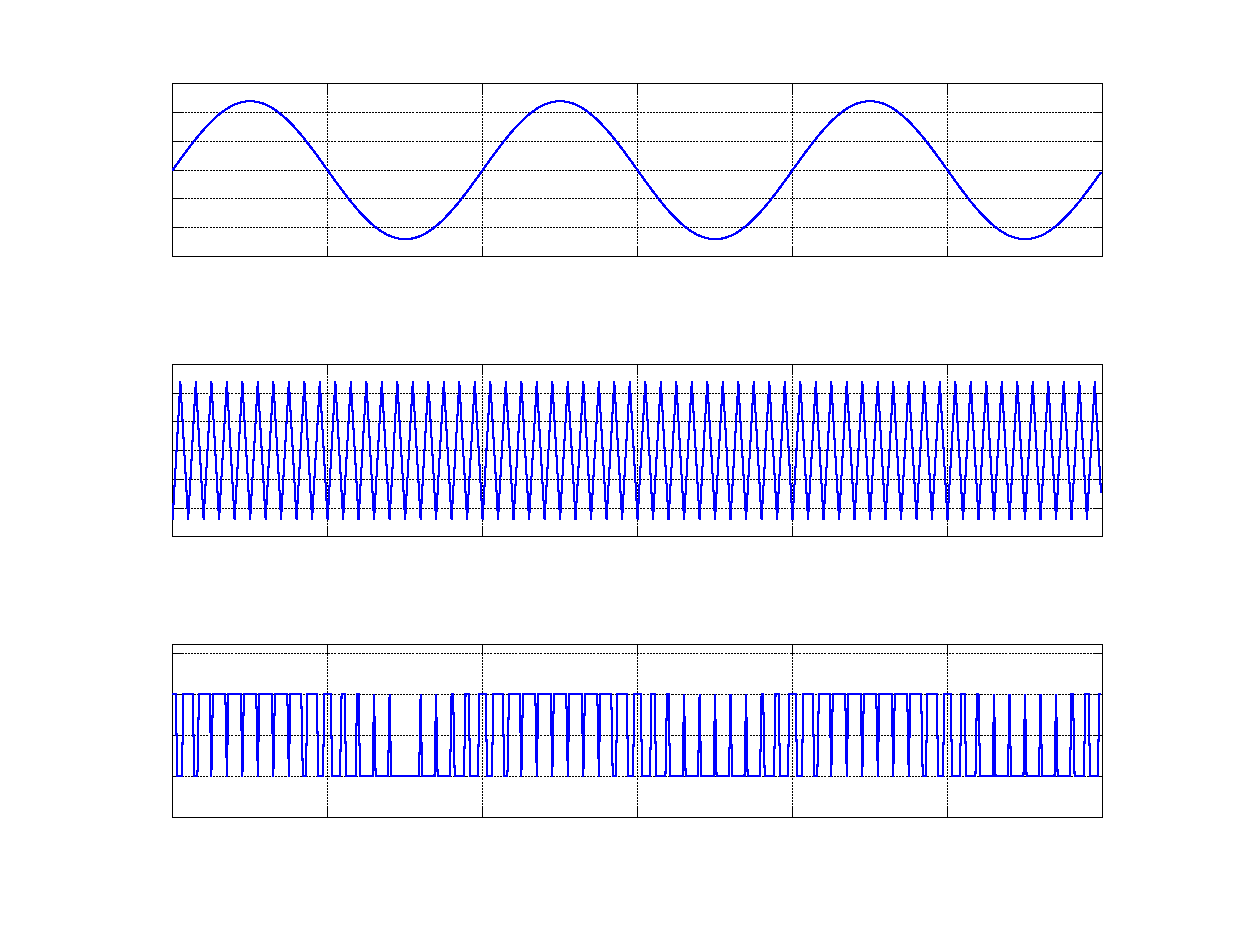
\includegraphics{pwm}}%
    \gplfronttext
  \end{picture}%
\endgroup
